\scanpage{40}
\mspage{\handwritten{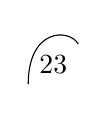
\begin{tikzpicture}[baseline=(p.base)]
\node[inner sep=1pt] (p) {23};
\draw ([xshift=-1mm,yshift=-1mm]p.south west) .. controls ([xshift=-1mm,yshift=3mm]p.north west) and ([xshift=2mm,yshift=3mm]p.north) .. ([xshift=1mm,yshift=1mm]p.north east);
\end{tikzpicture}}}
% archive sheet number: 39 (inverted, upper left)
% The two loop-and-stem signs below reproduce the handwritten linking marks; they are not read as letters.
% The top and bottom marginal continuations are placed at their marked insertion points.
sent en termes de limites projectives finies exclusivement, tandis que les autres notions impliquent implicitement des constructions faisant appel également à des limites inductives)\handwritten{\unsure{\begin{tikzpicture}[baseline=-.5ex,x=1ex,y=1ex]\draw (0,1.7) .. controls (.65,.7) and (.6,.15) .. (0,-.4);\end{tikzpicture}}}.
% The close-shaped pen trace may belong to the insertion boundary; its shape is retained without assigning punctuation.
\inserted{\handwritten{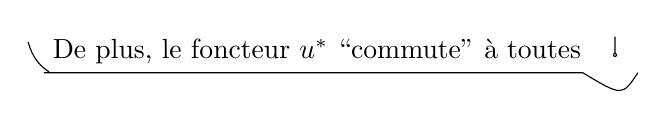
\begin{tikzpicture}[baseline=(plus.base)]
\node[inner sep=3pt] (plus) {De plus, le foncteur $u^{*}$ ``\uline{commute}'' à toutes\quad\tikz[baseline=-0.3ex,scale=.18]{\draw (0,1.3)--(0,.15) .. controls (-.4,-.2) and (.4,-.2) .. (0,.15);}};
\draw ([xshift=-2mm,yshift=1mm]plus.west) .. controls ([xshift=-1mm]plus.south west) and ([xshift=2mm]plus.south west) .. (plus.south west) -- ([xshift=-6mm]plus.south east) .. controls ([xshift=-1mm,yshift=-3mm]plus.south east) .. ([xshift=1mm]plus.south east);
\end{tikzpicture}
\figure{\begin{tikzpicture}
\node[inner sep=6pt,text width=.88\linewidth,align=left] (n) {\tikz[baseline=-0.3ex,scale=.18]{\draw (0,1.3)--(0,.15) .. controls (-.4,-.2) and (.4,-.2) .. (0,.15);}les opérations fonctorielles \deleted{\illegible{1}} habituelles faites en termes de telles structures, plus précisément à toutes les opérations qui \begin{tikzpicture}[baseline=(v.base)]
\node[inner sep=0pt] (v) {s'exprime\deleted{nt}\unsure{r}};
\node[anchor=south west,inner sep=0pt] (i) at ([yshift=2mm]v.north west) {\inserted{peuvent}};
\draw ([xshift=-1mm,yshift=-1mm]v.west) .. controls ([xshift=-2mm,yshift=3mm]v.west) and (i.south west) .. ([xshift=1mm,yshift=-1mm]i.south west) -- ([yshift=-1mm]i.south east) .. controls ([xshift=2mm]i.south east) .. ([xshift=2mm,yshift=1mm]i.south east);
\end{tikzpicture} en termes de $\varinjlim$ et de $\varprojlim$ finies: constructions d'objets libres (groupes ou modules libres, p.ex.) engendrés par un objet, produits tensoriels (cf. \S 6 plus bas) etc.};
\draw ([yshift=2mm]n.north west) .. controls ([xshift=-2mm]n.west) and ([xshift=-1mm]n.south west) .. (n.south west) -- ([xshift=1mm]n.south) -- ([xshift=2mm,yshift=2mm]n.south) -- ([yshift=2mm]n.south east);
\end{tikzpicture}}}}

% margin note slanted upward to the right
\margin{\handwritten{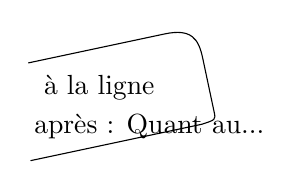
\begin{tikzpicture}[x=1cm,y=1cm]
\begin{scope}[rotate=12]
\node[anchor=west,inner sep=0pt] at (0,.45) {à la ligne};
\node[anchor=west,inner sep=0pt] at (-.22,0) {après : Quant au...};
\draw (-.12,.8)--(1.65,.8) .. controls (2,.8) and (2.06,.65) .. (2.06,.4)--(2.06,-.3) .. controls (2.06,-.4) .. (1.88,-.42)--(-.35,-.42);
\end{scope}
\end{tikzpicture}}}
% The opposing pen brackets mark the paragraph break immediately before Quant au.
\begin{tikzpicture}[baseline=(q.base)]
\node[inner sep=2pt] (q) {Quant au};
\handwritten{\draw ([xshift=-7mm]q.north west)--([xshift=-4mm,yshift=-.5mm]q.north west)--([xshift=-3mm]q.south west)--([xshift=-7mm,yshift=-1mm]q.south west);
\draw ([xshift=2mm]q.north east)--([xshift=-2mm]q.north west)--([xshift=-2mm]q.south west)--q.south east;}
\end{tikzpicture} foncteur image directe 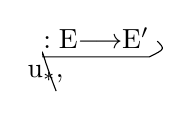
\begin{tikzpicture}[baseline=(d.base)]
\node[inner sep=0pt] (d) {$\mathrm{u}_{\handwritten{*}}$,};
\node[anchor=south west,inner sep=0pt] (i) at ([xshift=2mm,yshift=2mm]d.north west) {\inserted{$:\mathrm{E}\handwritten{\longrightarrow}\mathrm{E}'$}};
\handwritten{\draw ([xshift=-1mm,yshift=-1mm]d.south east) .. controls ([xshift=-3mm,yshift=3mm]d.east) and (i.south west) .. ([yshift=-1mm]i.south west) -- ([yshift=-1mm]i.south east) .. controls ([xshift=2mm]i.south east) .. ([xshift=1mm,yshift=1mm]i.south east);}
\end{tikzpicture} qui commute aux limites projectives, il ``respecte'' 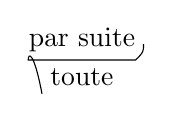
\begin{tikzpicture}[baseline=(b.base)]
\node[inner sep=0pt] (b) {toute};
\node[anchor=south,inner sep=0pt] (i) at ([yshift=2mm]b.north) {\inserted{par suite}};
\handwritten{\draw ([xshift=-1mm,yshift=-1mm]b.south west) .. controls ([xshift=-2mm,yshift=2mm]b.north west) and (i.south west) .. ([yshift=-1mm]i.south west) -- ([yshift=-1mm]i.south east) .. controls ([xshift=1mm]i.south east) .. ([xshift=1mm,yshift=1mm]i.south east);}
\end{tikzpicture} structure algébrique sur un objet (ou une famille d'objets) de $\mathrm{E}$, définissable en termes de limites projectives 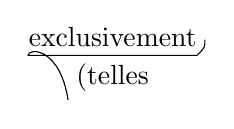
\begin{tikzpicture}[baseline=(b.base)]
\node[inner sep=0pt] (b) {(telles};
\node[anchor=south,inner sep=0pt] (i) at ([yshift=2mm]b.north) {\inserted{exclusivement}};
\handwritten{\draw ([xshift=-1mm,yshift=-1mm]b.south west) .. controls ([xshift=-2mm,yshift=2mm]b.north west) and (i.south west) .. ([yshift=-1mm]i.south west) -- ([yshift=-1mm]i.south east) .. controls ([xshift=1mm]i.south east) .. ([xshift=1mm,yshift=1mm]i.south east);}
\end{tikzpicture} les structures de groupe, d'anneau ou de module sur un anneau, \deleted{dans}\inserted{parmi} les exemples précédents). Par \unsure{
\begin{tikzpicture}[baseline=(a.base)]\node[inner sep=0pt] (a) {c};\node[inner sep=0pt] at ([xshift=.2pt,yshift=.25pt]a.center) {f};\end{tikzpicture}}ontre,
% Both f/c contours survive; their impression order is not established.
le foncteur $\mathrm{u}_{\handwritten{*}}$ n\deleted{e}'est en général pas exact à droite i.e. il ne commute pas en général aux limites inductives finies, et même ne transforme pas en général épimorphisme en épimorphisme\handwritten{\unsure{;|,}} (c'est d'ailleurs\begin{tikzpicture}[baseline=(x.base)]
\node[inner sep=0pt] (x) {\texttt{x}};
\node[inner sep=0pt,anchor=south west] at ([xshift=.2ex,yshift=-.2ex]x.north east) {\handwritten{\unsure{\begin{tikzpicture}[x=1ex,y=1ex]\draw (0,0)--(.25,.75);\end{tikzpicture}}}};
\end{tikzpicture}\deleted{\unsure{comme} nous le verrons au} ce défaut d'exactitude du foncteur $\mathrm{u}_{\handwritten{*}}$ qui est \handwritten{à} la source de ces propriétés cohomologiques, qui seront étudiées (du point de vue de l'algèbre homologique commutative) dans l'exposé suivant\handwritten{)}.
\inserted{\handwritten{Par suite, il ne \deleted{transforme pas}\inserted{s'étend pas}, en général,
\tikz[baseline=-.3ex,scale=.18]{\draw (0,0)--(.05,1.3) .. controls (-.35,1.65) and (.45,1.65) .. (.05,1.3);}
\figure{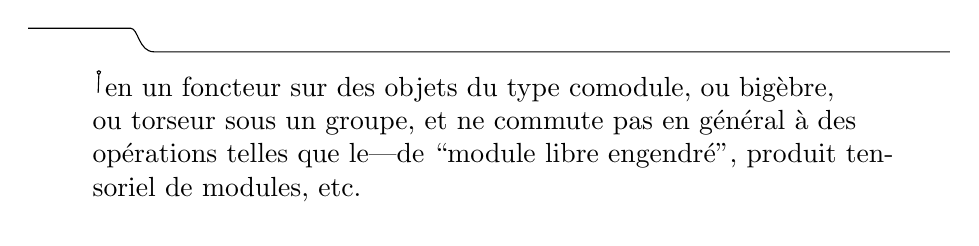
\begin{tikzpicture}
\node[inner sep=6pt,text width=.88\linewidth,align=left] (n) {\tikz[baseline=-.3ex,scale=.18]{\draw (0,0)--(.05,1.3) .. controls (-.35,1.65) and (.45,1.65) .. (.05,1.3);}en un foncteur sur des objets du type comodule, ou bigèbre, ou torseur sous un groupe\unsure{,} et ne commute pas en général à des opérations telles que \deleted{\unsure{le|de}} ``module libre engendré'', produit tensoriel de modules, etc.};
\draw ([xshift=-6mm,yshift=3mm]n.north west)--([xshift=7mm,yshift=3mm]n.north west) .. controls ([xshift=8mm,yshift=3mm]n.north west) and ([xshift=8mm]n.north west) .. ([xshift=10mm]n.north west)--(n.north east);
\end{tikzpicture}}}}

\deleted{2}\handwritten{3}.1.3. En pratique, lorsqu'on \deleted{se donne}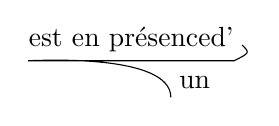
\begin{tikzpicture}[baseline=(b.base)]
\node[inner sep=0pt] (b) {un};
\node[anchor=south east,inner sep=0pt] (i) at ([xshift=3mm,yshift=3mm]b.north east) {\inserted{est \inserted{\handwritten{en}} présenced'}};
\handwritten{\draw ([xshift=-1mm,yshift=-1mm]b.south west) .. controls ([xshift=-1mm,yshift=3mm]b.north west) and ([xshift=1mm,yshift=-1mm]i.south west) .. ([yshift=-1mm]i.south west) -- ([yshift=-1mm]i.south east) .. controls ([xshift=2mm]i.south east) .. ([xshift=1mm,yshift=1mm]i.south east);}
\end{tikzpicture} foncteur $\mathrm{f}:\mathrm{E}\handwritten{\longrightarrow}\mathrm{F}$ d'un $\underline{\mathrm{U}}$-topos dans un autre, il y a lieu d'en expliciter 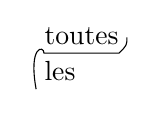
\begin{tikzpicture}[baseline=(b.base)]
\node[inner sep=0pt] (b) {les};
\node[anchor=south west,inner sep=0pt] (i) at ([yshift=2mm]b.north west) {\inserted{\handwritten{toutes}}};
\handwritten{\draw ([xshift=-1mm,yshift=-1mm]b.south west) .. controls ([xshift=-2mm,yshift=2mm]b.north west) and (i.south west) .. ([yshift=-1mm]i.south west) -- ([yshift=-1mm]i.south east) .. controls ([xshift=1mm]i.south east) .. ([xshift=1mm,yshift=1mm]i.south east);}
\end{tikzpicture} propri\unsure{
\begin{tikzpicture}[baseline=(a.base)]\node[inner sep=0pt] (a) {é};\node[inner sep=0pt] at ([xshift=.3pt,yshift=.2pt]a.center) {t};\end{tikzpicture}}\unsure{
\begin{tikzpicture}[baseline=(a.base)]\node[inner sep=0pt] (a) {t};\node[inner sep=0pt] at ([xshift=-.3pt,yshift=.2pt]a.center) {é};\end{tikzpicture}}és
% The two é/t superpositions are preserved without assigning an impression order.
d'exactitude, \deleted{y compris et de déterminer s'il admet un foncteur exact} y compris l'existence éventuelle de foncteurs adjoints à gauche ou à droite (cf. la note de bas de page précédente), pour parvenir à une compréhension de la ``nature géométrique'' de $\mathrm{f}$, \deleted{qui} compréhension qui sera généralement un guide indispensable pour 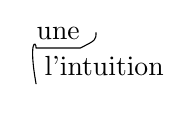
\begin{tikzpicture}[baseline=(b.base)]
\node[inner sep=0pt] (b) {\deleted{l'}intuition};
\node[anchor=south west,inner sep=0pt] (i) at ([xshift=-1mm,yshift=2mm]b.north west) {\inserted{une}};
\handwritten{\draw ([xshift=-1mm,yshift=-1mm]b.south west) .. controls ([xshift=-2mm,yshift=2mm]b.north west) and (i.south west) .. ([yshift=-1mm]i.south west) -- ([yshift=-1mm]i.south east) .. controls ([xshift=2mm]i.south east) .. ([xshift=2mm,yshift=1mm]i.south east);}
\end{tikzpicture} géométrique correcte de la situation. Ainsi, s'il s'avère que $\mathrm{f}$ commute aux limites inductives quelconques et aux limites projectives finies, il y a lieu d'écrire $\mathrm{f}$ sous la forme
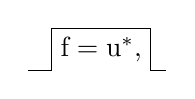
\begin{tikzpicture}[baseline=(n.base)]\node[inner sep=3pt] (n) {$\mathrm{f}=\mathrm{u}^{\handwritten{*}}$,};\handwritten{\draw ([xshift=-3mm]n.south west)--(n.south west)--(n.north west)--(n.north east)--(n.south east)--([xshift=2mm]n.south east);}\end{tikzpicture}
où
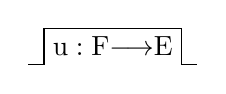
\begin{tikzpicture}[baseline=(n.base)]\node[inner sep=3pt] (n) {$\mathrm{u}:\mathrm{F}\handwritten{\longrightarrow}\mathrm{E}$};\handwritten{\draw ([xshift=-2mm]n.south west)--(n.south west)--(n.north west)--(n.north east)--(n.south east)--([xshift=2mm]n.south east);}\end{tikzpicture}
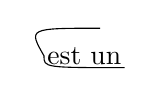
\begin{tikzpicture}[baseline=(n.base)]\node[inner sep=1pt] (n) {est un};\handwritten{\draw ([xshift=2mm,yshift=2mm]n.north) .. controls ([xshift=-2mm,yshift=2mm]n.north west) .. (n.west) .. controls (n.south west) .. (n.south east);}\end{tikzpicture}
morphisme de topos, i.e. d'interpréter $\mathrm{f}$ comme un foncteur ``image inverse'' par une ````application continue'' de topos. Lorsque $\mathrm{f}$ commute aux limites projectives quelconques, donc qu'il admet un adjoint à gauche,\deleted{$\mathrm{g}$}
\begin{tikzpicture}[baseline=(x.base)]\node[inner sep=0pt] (x) {\texttt{x}};\end{tikzpicture}
% Separate typewriter cancellation x in the following cell; not a further live variable.
